\PassOptionsToPackage{xetex}{xcolor}
\PassOptionsToPackage{xetex}{graphicx}
\documentclass[a4paper,landscape,headrule,footrule,xetex]{foils}

\input{headx.tex}

\usepackage{tikz}
\usepackage{tikz-dependency}
\usepackage{multicol}

\begin{document}
\header{Lecture 3}{Sentence meaning and compositionality}{}
\maketitle

%\include{schedule}


\myslide{Overview}

\begin{itemize}
\item Revision
\item Compositionality
\item Sentence Meaning
  \begin{itemize}
  \item Semantic Roles and Alternations
  \item Tense, Aspect, Modality and Evidentiality
  \end{itemize}
\item Close Reading and Word Sense Disambiguation
\end{itemize}

\section{Revision of Word Meaning}

\myslide{Word meaning}
\begin{itemize}
\item What is a word? How easy is it to define ‘word’?
\item Different ways of representing meaning
\item Lexical Relations
\item Derivational Relations
  \begin{itemize}
  \item Inchoative, causative, conative, \ldots (\txx{alternations})
  \item Agentive nouns
  \end{itemize}
\item Meaning: Relative or universal?
\end{itemize}

\myslide{Words} 
\begin{description}
\item \txx{word} slippery to define: orthographic, phonological, conceptual definitions mainly overlap
\item \txx{lexeme} base (uninflected) form of a word (or multi word expression)
\item \txx{vagueness} having an underspecified meaning
\item \txx{ambiguous} having more than one possible meaning
% \item \txx{content word} with a denotation (typically open class : \textbf{lexical word})
% \item \txx{function word} no denotation (typically closed class:
%   \textbf{grammatical word}, \textbf{structural word})
 \item \txx{Senses and Relations}
   
   \begin{description}
   \item \txx{polysemous} having multiple meanings
   \item \txx{monosemous} having just one meaning
   \item \txx{homonyms} words unrelated meaning; grammatically equivalent;
     with identical forms
\end{description} 
\end{description}

\myslide{Lexical Relations}
\begin{description}
\item \txx{synonymy}  all meanings identical; in all contexts; descriptive and non-
\item \txx{hyponymy} is-a, kind-of: supertype \textbf{hypernym}; subtype \textbf{hyponym}
\item \txx{meronymy} part-whole: part \textbf{meronym}; whole \textbf{holonym}
\item \txx{antonymy} (complementary, gradable, reverse, converse, taxonomic sisters)
\item \txx{member-collection} member of a group (\eng{tree-forest})
\item \txx{portion-mass} element of stuff (\eng{grain-rice})
\item \txx{domain}  used in a domain (\eng{[software] driver -golf})
\end{description}

\myslide{Wordnet}

\begin{itemize}
\item Defines words as linked semantic nets
\item Concepts are represented by synsets (synonym-sets)
\item Synsets have both definitions and semantic relations
\item We will use  \href{https://wordnet.princeton.edu/}{Princeton Wordnet} of English as our sense-inventory for projects one and two
\item Wordnets are available for many languages

\end{itemize}

\section{Compositionality}



\myslide{Meaning is built up}

\begin{itemize}
\item \txx{Compositional Semantics}: the meaning of the whole depends (only)
  on the meanings of the parts and the method of combination.
\item The hearer/reader's \txx{interpretation} brings in much more
  \begin{itemize}
  \item we bring in our existing knowledge
  \item we make inferences
  \end{itemize}
\item These inferences are based on (or constrained by) the semantics 
\item two central ideas \citep[formalized by: ][]{Katz:Fodor:1963}
  \begin{itemize}
  \item Semantic rules must be recursive to deal with infinite meaning
  \item Semantic rules interact with syntactic rules to build up meaning
  \end{itemize}
\item Two major components:
  \begin{itemize}
  \item A dictionary pairing lexical items with semantic representations
  \item A set of \txx{projection rules} that show how meaning is built up
  \end{itemize}
\end{itemize}

\myslide{Intersective Modification}

\begin{itemize}
\item Consider the simplest case of a noun and an adjective
  \begin{itemize}
  \item \lex{big} ``above average in size or number or quantity or magnitude or extent''
  \item \lex{head} ``the upper part of the human body or the front part of the body in animals; contains the face and brains''
  \end{itemize}
\item Each constrains the world, one picks out things that are
  ``big'' and the other things that ``are heads''.
\item Together \lex{big head} picks out things that have both properties: they
  are ``big'' and they ``have heads''.
\end{itemize}
\myslide{This is like intersection for sets}
\begin{center}
  \scalebox{2}{
    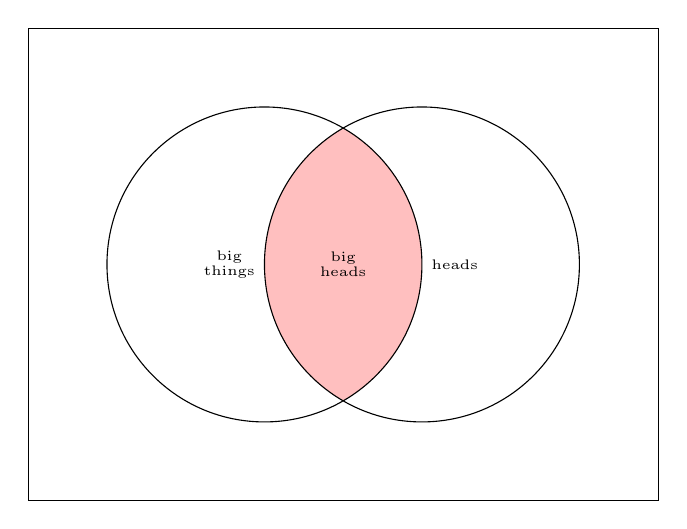
\begin{tikzpicture}
      \filldraw[fill=white] (-3,-3) rectangle (5, 3);
      \scope % A \cap B
      \clip (0,0) circle (2); \fill[pink] (2,0) circle (2);
      \endscope
      % outline
      \draw (0,0) circle (2) node [text=black,left,align=center] {\tiny\lex{big}\\ [-1.5ex] \tiny \lex{things}} 
      (2,0) circle (2) node [text=black,right] {\tiny\lex{heads}};
      \node[align=center] at (1,0) {\tiny \lex{big}\\[-1.5ex] \tiny \lex{heads}};
    \end{tikzpicture}} 
\end{center}

\begin{itemize}
\item This is the simplest form of composition
\end{itemize}

\myslide{Other kinds of intersective modification}

\begin{itemize}
\item \txx{Manner}: \eng{We \ull{live} very \ul{quietly}, sir} REDH
\item \txx{Restriction}: \eng{That trick of staining the fishes' scales of a delicate pink is quite \ull{peculiar} \ul{to China}} REDH
\item \txx{Location:} \eng{I would rather have my bracelets on him than on \ull{any criminal} \ul{in London}}
\item \txx{Time:} \eng{\ull{one day} \ul{in the autumn} \ul{of last year}}
\item \txx{State:} \eng{And \ull{sit} \ul{in the dark}}
\end{itemize}

The syntactic dependency (the fact that one word/phrase is associated
with another) helps us build the semantic model.  

\myslide{Some exceptions}

\begin{itemize}\addtolength{\itemsep}{-1ex}
\item Not all modification is intersective
  \begin{itemize}
  \item \eng{fake gun} is a thing like a gun: not a gun
  \item \eng{toy horse} is not a horse
  \item[?] come up with another example of non-intersective modification\task 
  \end{itemize}
  This requires different projection rules
\item Word combinations (\txx{multi-word expressions}) can pick up new
  meanings
  \begin{itemize}
  \item \eng{They have a big head} ``They are vain''
  \item \eng{They are a red head} ``They have red hair''
  \end{itemize}
  This requires a richer lexicon
\item There are many other ways of composing words (not just modification)
  \begin{itemize}
  \item Semantic roles: \eng{The dog barked}
  \item Intensification: \eng{They have a very big head}
  \item Embedding: \eng{I think they have a big head}
  \item Quantification: \eng{They have two heads/no head}
%  \item [\ldots]
  \end{itemize}
\end{itemize}


% \myslide{The dictionary}
% \MyLogo{Similar to \txx{genus} and \txx{differentiae}.}
% \begin{itemize}
% \item \lex{bachelor} \{N\}
%   \begin{enumerate}
%   \item \izb{human} \izb{male} [one who has never been married]
%   \item \izb{human} \izb{male} [young knight serving under the standard of another knight]
%   \item \izb{human} [one who has the lowest academic degree]
%   \item \izb{animal} \izb{male} [young fur seal without a mate in the breeding season]
%   \end{enumerate}
% \item \izb{semantic markers} are the links that bind lexical items
%   together in lexical relations
% \item {[\txx{distinguishers}]} serve to identify this particular lexical item
%     \\ this information is not relevant to syntax
% \end{itemize}

\myslide{Projection Rules}
\MyLogo{More about this in Theories of Syntax/HPSG}

\begin{enumerate}
\item Projection rules combine with syntactic rules to produce the
  meaning of a sentence
  \\ these can be grouped together in \txx{signs} or \txx{constructions}
  \begin{itemize}
  \item Information is built up as we parse a sentence
    \begin{itemize}
    \item Information is only added, never deleted
    \item It must come from words or rules (or constructions)
    \end{itemize}
  \end{itemize}
\item Different languages show these combinations in different ways
  \begin{itemize}
  \item English primarily uses word order
  \item Japanese uses case-marking
  \item [\ldots{}]
  \end{itemize}
\item[?] Consider \eng{a very stout, florid-faced, elderly gentleman,
    with fiery red hair}
  \begin{itemize}
  \item How many examples of intersective modification are there here?\task
  \item Can you describe the other relations involved?\task
  \end{itemize}
  
% \item \txx{Selectional restrictions} \sr{} help to reduce ambiguity and
%   limit the possible readings
\end{enumerate}

% \myslide{Selectional restrictions} 

% \MyLogo{Modern theories prefer \txx{selectional preferences}:
%   probabilities not categories.}
% \begin{enumerate}
% \item \lex{colorful} \{adj\}
%   \begin{enumerate}
%   \item\label{A} \izb{color} [abounding in contract or variety of bright colors) 
%     \sr{\izb{physical object} or \izb{social activity}}
%   \item\label{B} \izb{evaluative} [having distinctive character, vividness or picturesqueness) 
%     \sr{\izb{aesthetic object} or \izb{social activity}}
%   \end{enumerate}

% \item \lex{ball} \{N\}
%   \begin{enumerate}
%   \item\label{D} \izb{social activity} \izb{large} \izb{assembly} [for the purpose of social dancing]
%   \item\label{E} \izb{physical object} [having globular shape]
%   \item\label{F} \izb{physical object} [solid missile for project by engine of war]
%   \end{enumerate}
% \end{enumerate}
% \begin{itemize}
% \item \eng{colorful ball}: The selectional restrictions rule out: \ref{B} $+$ \ref{E},  \ref{B} $+$ \ref{F}
% \end{itemize}


\myslide{Completion}

\begin{itemize}
\item When we listen (or read) we actively anticipate the next word
  (or words)
\item We can guess them fairly well
  \begin{itemize}
\item \eng{Recognising, as I do, that you are the second highest
    expert in Europe-'}
\item \eng{'Indeed, sir! May I inquire who has the honour to be the
    first?' asked Holmes, with some asperity.} \ldots
  \item \eng{But as a practical man of affairs it is acknowledged that
      you stand alone. I trust, sir, that I have not inadvertently-'}
  \item \eng{'Just a little,' said Holmes. '}
  \end{itemize}
\item What is missing here?\task

\end{itemize}


\section{Sentence Meaning}


\myslide{Situations}

\begin{itemize}
\item Noun phrases refer to entities
\item Sentences refer to situations
  \begin{itemize}
  \item Situations can be constrained in various ways
  \item What is the event in question?
  \item Who participates in it?
  \item When did it happen?
  \item Is it ongoing or has it finished?
  \item Is our knowledge of it certain?
  \end{itemize}
\item The core of an event is typically represented by a verb or
  adjective 
  \begin{itemize}
  \item Verbs typically refer to actions (but can refer to states)
    \\ \eng{He \ul{stepped} swiftly forward \ldots} DANC
    \\  \eng{I \ul{know} you, you scoundrel!} DANC
  \item Adjectives typically refer to states
    \\ \eng{Your sister is \ul{dead}, then?} DANC
  \end{itemize}
\end{itemize}

\myslide{Semantic  Roles}
\MyLogo{The set of roles we use is from \citet[Chapter~6]{Saeed:2009}.}
In this section we talk about the relations between the participants
in a situation and the situation itself.

\begin{itemize}
\item  \txx{Semantic roles} are parts of the sentence that 
correspond to the participants in the situation 
described

\item  They classify relations between entities in a situation
\\[2ex] \begin{dependency}
\begin{deptext}[column sep=1em]
He \& seized \& the poker, \& and \& bent \& it \& into \& a curve \ldots \\ %with his huge brown hands.}
\end{deptext}
\deproot[edge unit distance=2.5ex]{2}{ROOT}
\depedge{1}{2}{AGENT}
\depedge{3}{2}{PATIENT}
\depedge{1}{5}{AGENT}
\depedge{6}{5}{PATIENT}
\depedge{7}{6}{GOAL}
\end{dependency}
 
\item  Also known as
\begin{itemize}
\item  Deep case \citep{Fillmore:1968}
\item  Thematic roles; Theta roles;   $\theta$-roles
\item  Participant Roles
\end{itemize}
\end{itemize}
 
\myslide{Roles link different alternations}
\begin{exe}
  \ex\eng{Kim patted Sandy}
  \ex\eng{Sandy was patted by Kim}
\end{exe}
\begin{itemize}
\item The semantic roles are different from the grammatical relations.
\item Which is the \txx{subject} and which the \txx{object} in these sentences?
\item What are the semantic roles of Kim and Sandy?
\item \txx{semantic dependencies}: An abstract representation of the meaning links word-senses to
  each other using semantic roles: different sentences may end up the same at this level
\\[2ex] \begin{dependency}
\begin{deptext}[column sep=1em]
Kim \& pat$_1$ \& Sandy \\ %with his huge brown hands.}
\end{deptext}
\deproot[edge unit distance=1.5ex]{2}{ROOT}
\depedge{1}{2}{AGENT}
\depedge{3}{2}{PATIENT}
\end{dependency}

\end{itemize}

\myslide{Semantic Roles}
\MyLogo{Some prose and examples from \citet{Bender:2013}}
\begin{itemize}
\item \txx{AGENT} (takes \eng{deliberately, on purpose, what did X do?})
  \begin{quote}
    A participant which the meaning of the verb specifies as doing or causing something,
    possibly intentionally. 
  \end{quote}
  \begin{itemize}
  \item The initiator, performer of controller of an action; typically volitional, typically animate
  \item Typically \textsc{subject}
  \end{itemize}
  \begin{exe}
      \ex\eng{\eng{\ul{Kim} kicked Sandy}}
      \ex\eng{\eng{\ul{The ogre} leaped into the fray}}
      \ex\eng{\eng{\ul{The student} watched the video}}
    \end{exe}
\item (\txx{ACTOR}) generalization of \txx{AGENT} that allows non-volitional, non-actor
  \\ if you use this, then \txx{AGENT} is restricted to animate, volitional participants
\item Find an example of AGENT in \Story{}\task
\newpage
\item  \txx{PATIENT} (\eng{What happened to X?})
  \begin{quote}
    A participant which the verb characterizes as having something
    happen to it, and as being affected by what happens to it.
    %Examples: objects of kill, eat, smash but not those of watch, hear
    %and love.
  \end{quote}
  \begin{itemize}
  \item The undergoer of an action
  \item  Undergoes change in state usually, both animate and 
    inanimate
  \item Typically \textsc{object}
  \end{itemize}
  \begin{exe}
    \ex\eng{\eng{Kim kicked \ul{Sandy}}}
    \ex\eng{\eng{The ogre ate  \ul{the dog}}}
    \ex\eng{$^\#$\eng{The student watched \ul{the video}}}
    \ex\eng{$^\#$\eng{I heard \ul{a sound}}}
  \end{exe}
\item Find an example of PATIENT in \Story{}\task
\newpage
\item  \txx{THEME}
  \begin{quote}
     A participant which is characterized as changing its position or condition, or as
being in a state or position. 
  \end{quote}
  \begin{itemize}
  \item  Moved, location or state is described
  \item Typically \textsc{object}
\end{itemize}
\begin{exe}
  \ex \eng{\eng{Hiromi put \ul{the book} on the shelf}}
  \ex \eng{\eng{Freddy gave you \ul{the chocolate}}}
  \ex \eng{\eng{\ul{The book} is on the shelf}}
  \ex \eng{\eng{\ul{The protagonist} died}}
  \ex *\eng{\eng{\ul{The dog} walked home}}
\end{exe}
\item Find an example of THEME in \Story{}\task
\newpage

\item  \txx{EXPERIENCER}
  \begin{quote}
    A participant who is characterized as aware of something.
  \end{quote}
  \begin{itemize}
  \item   Non-volitional, displaying awareness of action, state
  \item Typically \textsc{subject}
  \end{itemize}
  \begin{exe}
  \ex\eng{\ul{Liling} heard thunder}
  \ex\eng{\ul{Jo} felt sick}
  \ex\eng{The lecturer annoyed \ul{the students}}
\end{exe}
\item Find an example of EXPERIENCER in \Story{}\task
\newpage
\item  \txx{BENEFICIARY}
  \begin{itemize}
  \item   for whose benefit the action was performed
  \item   Typically indexed by "for" PP in English
    \\ or \textsc{object} in ditransitive verbs
  \end{itemize}
  \begin{exe}
  \ex\eng{They made \ul{me} a present}
  \ex\eng{They made a present \ul{for me}}
\end{exe}

\item  \txx{LOCATION}
  \begin{itemize}
  \item  Place
  \item Typically indexed by locative PPs in English
  \end{itemize}
  \begin{exe}
  \ex\eng{I am living \ul{in Indonesia}}
  \ex\eng{It is \ul{on the table}}
\end{exe}
\item Find  examples of BENEFICIARY and LOCATION in \Story{}\task
\newpage  

\item  \txx{GOAL}
  \begin{itemize}
  \item  towards which something moves (lit or metaphor)
 \item  Typically indexed by "to" PP in English 
   \\ or \textsc{object} in ditransitive
  \end{itemize}
  \begin{exe}
  \ex\eng{She handed the form \ul{to him}}
  \ex\eng{She handed \ul{him} her form}
  \end{exe}
\item  \txx{SOURCE}
 \begin{itemize}
 \item  from which something moves or originates
 \item  Typically indexed by "from" PP in English
 \end{itemize}
  \begin{exe}
 \ex\eng{We gleaned this \ul{from the Internet}}  
\end{exe}
\item Find  examples of SOURCE and GOAL in \Story{}\task
\newpage
\item  \txx{STIMULUS}
  \begin{itemize}
  \item  Usually used in connection with EXPERIENCER
  \end{itemize}
  \begin{exe}
  \ex\eng{\ul{The lightning} scared them}
  \ex\eng{I don't like \ul{the lightning}}
\end{exe}
\item  \txx{INSTRUMENT/MANNER}
  \begin{itemize}
  \item  Means by which action is performed
  \item  Can be indexed by "with" PP in English
  \end{itemize}
  \begin{exe}
    \ex\eng{I ate breakfast \ul{with chopsticks}}
  \end{exe}
\item Find  examples of STIMULUS and INSTRUMENT in \Story{}\task
\end{itemize}


\myslide{PropBank Roles}

\begin{itemize}
\item An influential set of semantic roles comes from  PropBank \citep{Palmer:Gildea:Kingsbury:2005}
\item They have 6 core roles and 17 modifier roles
\item The core roles, meaning is defined per verb sense \\
  \begin{tabular}{lll}
    Role & Description & Example \\
    ARG0 & agent          & \\
    ARG1 & patient   & \\
    ARG2 & instrument, benefactive, attribute   & \\
    ARG3 & starting point, benefactive, attribute   & \\
    ARG4 & ending point   & \\
    ARGA & secondary agent & \eng{\ul{Kim}$_A$ \ull{trotted} \ul{her horse}$_0$}
      \end{tabular}
    \item \lex{seize.01} ``acquire (forcefully or stealthily)''
    \\  \begin{tabular}{ll}
        Arg0-PAG: &agent, entity acquiring something\\
        Arg1-PPT: &thing acquired \\
        Arg2-DIR: &acquired-from
      \end{tabular}
      \\[1.5ex] \eng{\ul{Sandy}$_0$ \ull{seized} \ul{the poker}$_1$ \ul{from Kim}$_2$}
    \end{itemize}


\myslide{The Modifier Roles}
\MyLogo{Can be used with any verb}
\begin{small}
\begin{verbatim}
COM: Comitative
LOC: Locative
DIR: Directional
GOL: Goal
MNR: Manner
TMP: Temporal
EXT: Extent
REC: Reciprocals
PRD: Secondary Predication
PRP: Purpose
CAU: Cause
DIS: Discourse
ADV: Adverbials
ADJ: Adjectival
MOD: Modal
NEG: Negation
DSP: Direct Speech
LVB: Light Verb
CXN: Construction
\end{verbatim}
  \end{small}

\myslide{Some Issues}
\begin{itemize}
\item  Every theory has a different set of roles
\item  It is hard to generalize: roles can be very word specific
\item  Roles are very under-specified, these are all PATIENT!
\begin{exe}
\ex\eng{The genie touched \ul{the lamp} with their nose.}
\ex\eng{The baby rubbed \ul{the lamp} with its hands.}
\ex\eng{The baby squeezed \ul{the rubber toy} with its hands.}
\ex\eng{She cracked \ul{the mirror} with a stone.}
\end{exe}
\end{itemize}



\myslide{Linking Grammatical Relations and Semantic Roles}
\begin{itemize}
\item    Semantic roles typically map onto grammatical 
  functions systematically
  \begin{itemize}
  \item  AGENT is usually the subject
  \item  PATIENT is usually the object
  \end{itemize}
\item  It is possible to predict how arguments are linked to 
the verb from their semantic roles, and hence their 
grammatical functions.
% \end{itemize}

\item Many verbs allow alternations ``syntactic variants with different roles''

\begin{exe}
  \ex \eng{Jo broke the ice with a pickaxe}  \sr{AGENT, PATIENT, INSTRUMENT}
  \ex \eng{The pickaxe broke the ice}  \sr{INSTRUMENT, PATIENT}
  \ex \eng{The ice broke}  \sr{PATIENT}
\end{exe}
\end{itemize}

\myslide{Other Predicates}

\begin{itemize}
\item Adjectives  (normally theme)
  \begin{exe}
  \ex \eng{John is tall} (THEME)
  \ex \eng{John is cold [to touch]} (THEME)
  \ex \eng{John is/feels cold} (EXPERIENCER)
    \\ different adjectives in e.g., Japanese:
    \\  \eng{冷たい} \jpn[cold (to touch)]{tsumetai}  vs \eng{寒い} \jpn[(feel) cold]{samui}
  \end{exe}
\item Predicative Copula (treat second NP as predicate)
  \begin{exe}
  \ex \eng{John is a boy} (THEME)
  \end{exe}
\item Identity Copula (reversible)
  \begin{exe}
  \ex \eng{Kim is my teacher} (THEME, THEME)?
  \ex \eng{My teacher is Kim} (THEME, THEME)?
  \end{exe}


\end{itemize}



% \myslide{Thematic Hierarchy}

% \begin{itemize}
% \item  The higher you are in the hierarchy the more likely 
% to be subject (then object, then indirect, then 
% argument PP, then adjunct PP)
% \end{itemize}
% \[  \mbox{AGENT} > 
% \left\{\begin{array}[c]{l} \mbox{GOAL/RECIPIENT} \\ \mbox{BENEFICIARY} \end{array} \right\}  >
% \left\{\begin{array}[c]{l} \mbox{THEME} \\ \mbox{PATIENT} \end{array} \right\}  >
% \mbox{INSTRUMENT} > 
% \mbox{LOCATION} \]

% \begin{itemize}
% \item  Generally true across languages
% \end{itemize}



% \myslide{Dowty's Proto-Arguments}
% \MyLogo{\citet{Dowty:1991}}
% \begin{itemize}
% \item  The \txx{Agent} Proto-Role 
% \begin{itemize}
% \item  Volitional
% \item  Sentient (and/or perceptive)
% \item  Causes event or change of state; 
% \item  Movement
% \end{itemize}
% \item  The \txx{Patient} Proto-Role
% \begin{itemize}
% \item  Change of state
% \item  Incremental theme (i.e. determines aspect)
% \item  Causally affected by event
% \item  Stationary (relative to movement of proto-agent).     
% \end{itemize}
% \end{itemize}

% \myslide{Dowty's Argument Selection Principle}
% \begin{itemize}
% \item   when a verb takes a subject and an object
%   \begin{itemize}
%   \item  the argument with the greatest number of Proto-Agent 
%     properties will be the one selected as \textsc{subject}
%   \item  the one with the greatest number of Proto-Patient properties 
%     will be selected as \textsc{object}
%   \end{itemize}
% \item   Try: \lex{threw} --- ball, the man, the dog

% \item   Relatively predictive, but what about sentences 
% such as:
% \\  \eng{The hunger killed him}?
% \end{itemize}


\myslide{Alternations}
\begin{itemize}
\item  Many verbs have multiple possible mappings of grammatical function to role
  \begin{exe}
    \ex
    \begin{xlist}
      \ex\eng{Kim broke the window with the hammer}
      \ex\eng{The hammer broke the window}
      \ex\eng{The window broke}
    \end{xlist}
    \ex
    \begin{xlist}
      \ex\eng{I cut the cake with the knife}
      \ex\eng{This cake cuts easily}
    \end{xlist}
  \end{exe}  
\item  The relations between them are called \txx{alternations}
\item  English Verb Classes and Alternation \citep{Levin:1993}
\end{itemize}


\myslide{There are many alternations}
%\MyLogo{These are also alternations for Levin}
\begin{itemize}
\item  A common  way to change the number of arguments is called 
\txx{voice}: passive, middle
\begin{exe}
  \ex \txx{Transitive Passive}
  \begin{xlist}
    \ex\eng{Kim ate Sandy}
    \ex\eng{Sandy was eaten (by Kim)}
  \end{xlist}
  \ex \txx{Ditransitive Passive} 
  \begin{xlist}
    \ex\eng{Abraham gave Brown chocolate}
    \ex\eng{Abraham gave chocolate to Brown}
    \ex\eng{Chocoloate was given to Brown (by Abraham)}
    \ex\eng{Brown was given chocolate (by Abraham)}
  \end{xlist}
\newpage
  \ex \txx{Transitive Middle} (or just causative/inchoative)
  \begin{xlist}
    \ex\eng{They open the gate very quietly}
    \ex\eng{The gate opens very quietly}
  \end{xlist}
  \ex \txx{Intransitive Middle}
  \begin{xlist}
    \ex\eng{The knife cuts the cake well}
    \ex\eng{The knife cuts well}
  \end{xlist}
\end{exe}
\item But there are many other alternations:
\begin{exe}
\ex \txx{Conative} alternation:
\begin{xlist}
    \ex\eng{Kim \ul{hit} the door} $\leftrightarrow$ \eng{Kim \ul{hit} at the door}
  \end{xlist}
\ex \txx{Body-part possessor ascension} alternation:
  \begin{xlist}
    \ex\eng{Kim \ul{cut} Sandy's arm} $\leftrightarrow$ \eng{Kim \ul{cut} Sandy on the arm}
  \end{xlist}

\end{exe}
%\item Can you find 
\end{itemize}

\myslide{Why so many possibilities?}

\begin{itemize}
\item So we can emphasize different participants
\item We may not know all the participants
\item We may not care about all the participants
\item There are also lexical alternations
\end{itemize}
\begin{exe}
\ex \eng{Kim \ul{killed} Sandy} vs \eng{Sandy \ul{dies}}
\ex c.f. \eng{Kim \ul{melted} the ice} vs \eng{the ice \ul{melted}}
\ex \glll 金が 氷を \ul{溶かした}  {~~~vs~~~}  氷が \ul{溶けた} \\ 
Kim-ga koori-wo \ul{tokashita}  {} koori-ga \ul{toketa} \\
  Kim-\textsc{sbj} ice-\textsc{obj} \textit{melt:trans} 
{} ice-\textsc{sbj} \textit{melt:intrans} \\
\end{exe}



%%%
%%% TAM lec 05
%%%
\myslide{Video}
\MyLogo{Comitative or Instrument}
\begin{itemize}
\item \textit{I want to cook \ul{with} you}  IT Crowd, Series 2 - Episode 3
\\ \url{https://www.youtube.com/watch?v=gOE-q20RcDM}
\begin{verbatim}
Moss    Look, I've got your advert here.
        I printed it out.
        I want to cook with you.
Johann  No, my English is not so good 
Moss    You want to cook with me, using me, you mean.
Johann  Ah yes! Yes.
        You see.
Moss    I see where the confusion was.
        I thought this was a cookery course.
        But you wanted someone who would agree to let you kill and eat them.
Johann  Ja! You see? 
Moss    That is funny.
Johann  So you're not interested? 
Moss    No, thanks, it's not for me.
Johann  How disappointing.
\end{verbatim}
\end{itemize}


\section{Tense, Aspect and Modality (TAM)}

\myslide{TAM}
\begin{itemize}
\item  We need to distinguish grammatical expression from 
  meaning
  \begin{itemize}
  \item  Tense vs Time
  \item  Grammatical Aspect vs Semantic Aspect
  \item  Mood vs Modality
  \item  Surface Case vs Deep Case
  \end{itemize}
\item  The relation between them is refered to as
  \begin{itemize}
  \item  linking; syntax-semantics interface; grammar
  \end{itemize}
\end{itemize} 
 

\myslide{How Universal is Tense?}
\begin{itemize}
\item  Grammatical tense is different from semantic time
\item  English has \iz{past/non-past}
\item  Latin marks \iz{past/present/future}
\item  Chibemba (Bantu) has \txx{metrical tense}
  \begin{multicols}{2}
  \begin{itemize}
  \item  Remote Past ($<$ yesterday)
  \item  Removed Past (yesterday)
  \item  Near Past (today)
  \item  Immediate Past (past few hours)
  \item Immediate Future (next few hours)
  \item Near Future (today)
  \item Removed Future (tomorrow)
  \item Remote Future ($>$ tomorrow)
  \end{itemize}
\end{multicols}
\end{itemize}

\myslide{Tense and Time}
\begin{itemize}
\item  Locate a situation to with respect to a point in time
  \begin{itemize}
  \item  S = speech point
  \item  R = reference time
  \item  E = event time
  \end{itemize}
\item   Hans Reichenbach (1947)
\item Simple Tense
\begin{itemize}
\item  Past ($R = E < S$) \eng{saw} \hfill
\begin{tabular}[t]{ccc|ccc|ccc}
  \mc{3}{c}{past} &  \mc{3}{c}{present} & \mc{3}{c}{future} \\
&R=E&&&S&&&& \\ \hline
&&&&&&& \\ 
\end{tabular}
\item  Present ($R = S = E$) \eng{see} \hfill
\begin{tabular}[t]{ccc|ccc|ccc}
  \mc{3}{c}{past} &  \mc{3}{c}{present} & \mc{3}{c}{future} \\
&&&&S=R=E&&&&  \\ \hline
&&&&&&& \\ 
\end{tabular}
\item  Future ($S < R = E$) \eng{will see}\hfill
\begin{tabular}{ccc|ccc|ccc}
  \mc{3}{c}{past} &  \mc{3}{c}{present} & \mc{3}{c}{future} \\
&&&&S&&&R=E& \\ \hline
&&&&&&& \\ 
\end{tabular}
\end{itemize}
\end{itemize}
\myslide{Complex Tense}

\begin{itemize}
\item  Past Perfect ($E < R < S$) \eng{had seen} \hfill
\begin{tabular}[t]{ccc|ccc|ccc}
  \mc{3}{c}{past} &  \mc{3}{c}{present} & \mc{3}{c}{future} \\
E&R&&&S&&&& \\ \hline
&&&&&&& \\ 
\end{tabular}
\\ \eng{By 1939 my Father had seen many arrests}
\item  Future Perfect ($S< E < R$) \eng{will have seen} \hfill
\begin{tabular}[t]{ccc|ccc|ccc}
  \mc{3}{c}{past} &  \mc{3}{c}{present} & \mc{3}{c}{future} \\
&&&&S&&&E&R \\ \hline
&&&&&&& \\ 
\end{tabular}
\\ \eng{By 2039 my son will have seen many things}
\end{itemize}

\myslide{Aspect in English}
\begin{itemize}
\item  Finer grained talking about time!
\item  \txx{Progressive}  is used for ongoing processes (unfinished)
  \begin{itemize}
  \item  \txx{Past Progressive} \eng{I was building the building}
  \item  \txx{Present Progressive} \eng{I am building the building}
  \item  \txx{Future Progressive} \eng{I will be building the building}  %(E < R = S) ???
  \end{itemize}
\item  \txx{Perfect} compares the time to the reference point
 \begin{itemize}
  \item  \txx{Past Perfect} \eng{I had built the building} ($E<R<S$)
  \item  \txx{Present Perfect} \eng{I have built the building}  ($E<R=S$)
  \item  \txx{Future Perfect} \eng{I will have built the building}  ($S<E<R$)
  \end{itemize}
\end{itemize}

\myslide{Aspect more Generally}

\begin{itemize}
\item  \txx{Perfective} focuses on the end point
  \begin{itemize}
  \item  \txx{Completive} \eng{I built the building}
  \item  \txx{Experiential} \eng{I have built the building} %(E < R = S) ???
  \end{itemize}
\item  \txx{Imperfective} 
  \begin{itemize}
  \item  \txx{Progressive} \eng{I was listening/I am listening}
  \item  \txx{Habitual} \eng{I listen to the Goon Show}
\end{itemize}
\item Different languages grammaticalize different things
\end{itemize}

% \item  Progressive
% \item  Habitual
% \item  Completive
% \item  Experiential

\myslide{Mood and Modality}
\begin{itemize}
\item  Modality expresses varying degrees of the speaker's 
commitment and belief
\item In English it is typically expressed by an auxiliary verb.
\begin{exe}
  \ex \eng{She \ul{has} left by now.}
  \ex \eng{She \ul{must} have left by now.}
  \ex \eng{She \ul{could} have left by now.}
  \ex \eng{She \ul{needn't} have left by now.}
  \ex \eng{She \ul{couldn't} have left by now.}
  \ex \eng{She \ul{has} to leave by now.}
  \ex \eng{She \ul{must} leave by now.}
  \ex \eng{She \ul{can} leave now. }
\end{exe}
\end{itemize}

\myslide{Other means of expression}
\begin{itemize}
\item Explicit External Verb
  \begin{exe}
    \ex \eng{I \ul{know} that $S$}
    \ex \eng{I \ul{believe} that $S$}
  \end{exe}
\item Adverb or Adjective
  \begin{exe}
    \ex \eng{It is \ul{certain that} $S$}
    \ex \eng{It is \ul{likely that} $S$}
    \ex \eng{I will \ul{probably} $S$}
    \ex \eng{I will \ul{definitely} $S$}
  \end{exe}

\end{itemize}

\myslide{Knowledge vs Obligation}
\begin{itemize}
\item  \txx{Epistemic modality}: Speaker signals degree of  
knowledge.
\begin{exe}
  \ex \eng{You can drive this car} \cmm{You are able to}
\end{exe}
\item  \txx{Deontic modality}: Speaker signals his/her attitude  
to social factors of obligation and permission.
\begin{itemize}
\item \txx{Permission}
  \begin{exe}
    \ex \eng{You can drive this car}  \cmm{You have permission to}
    \ex \eng{You may drive this car}  
  \end{exe}
\item \txx{Obligation}
  \begin{exe}
    \ex \eng{You must drive this car}  \cmm{You have an obligation to}
    \ex \eng{You ought to drive this car} 
  \end{exe}
% \item  Question: How do you use `must', `confirm', and 
% `sure' in Singlish? ???
\end{itemize}
\item [?] Find examples of each type (auxiliary, verb, adverb/adjective) in \Story{}\task
\item [?] Determine whether they are deontic or epistemic\task
\end{itemize}

\myslide{Possible Worlds}

\begin{itemize}
\item We can analyze these in terms of \txx{possible worlds}

\item We mark how close a hypothetical case is to reality:
  \begin{exe}
    \ex \eng{It must be/might be/is/can't be \ul{hot outside}}
  \end{exe}
  And model it as the degree of overlap of the worlds
\item Similarly for \txx{conditionals} (condition/consequence)
  \begin{exe}
    \ex \eng{If it is Singapore, it will be hot outside}
    \ex \eng{If it were Singapore, it would be hot outside}
    \ex \eng{If you should go to Singapore, take some cool clothes}
  \end{exe}
\end{itemize}

% \myslide{Real vs Hypothetical}
% \begin{itemize}
% \item  \txx{Realis} is used for things that occur
% \item  \txx{Irrealis} is used for things that are not claimed to 
% occur (hypotheticals, negation, future)
% \item  English doesn't mark this normally
%   \begin{exe}
%     \ex \eng{If I were to go} \textnormal (subjunctive)
%   \end{exe}
% \item  What about Singlish? ???
%  \begin{exe}
%     \ex \eng{I got go.}
%     \ex \eng{I sure confirm go.}
%     \ex \eng{I maybe go.}
%   \end{exe}
% \end{itemize}

\myslide{Mood more Generally}
\MyLogo{See \citet{Saeed:2009} for more examples}
\begin{itemize}
\item Grammatical Inflection used to mark modality is called \txx{mood}
  \begin{itemize}
  \item \txx{indicative} expresses factual statements
  \item \txx{conditional} expresses events dependent on a condition
  \item \txx{imperative} expresses commands
  \item \txx{injunctive} expresses pleading, insistence, imploring
  \item \txx{optative} expresses hopes, wishes or commands 
  \item \txx{potential} expresses something likely to happen
  \item \txx{subjunctive} expresses  hypothetical events; opinions or emotions
  \item \txx{interrogative} expresses questions
\end{itemize}
\item In English most things are marked syntactically: \vspace*{-1ex}
    \begin{exe}
      \ex  \eng{I \ul{am} good}  \hfill indicative
      \ex  \eng{\ul{Am} I good?} \hfill interrogative
    \ex \eng{\ul{Be} good!} \hfill imperative
    \ex \eng{If I \ul{were} a rich man} \hfill subjunctive
  \end{exe}
\item [?] Find examples of non-indicative sentences in \Story{}\task
\end{itemize}

\myslide{Evidentiality}
\MyLogo{Skip if too long}
\newcommand{\TIPA}[1]{\textipa{\mtcitestyle{#1}}}

\begin{itemize}
\item  Some languages must show you gained the evidence
\\item  \txx{nonvisual sensory}:  speaker felt the sensation
  \begin{itemize}
  \item \ipa{/pʰa·békʰ-\ul{ink’e/}} ``burned, I felt it''
  \end{itemize}
\item  \txx{inferential}: speaker saw circumstantial evidence 
  \begin{itemize}
  \item  \ipa{/pʰa·bék-\ul{ine}/}  ``must have burned''
  \end{itemize}
\item  \txx{hearsay (reportative)}:   speaker is reporting what was told
  \begin{itemize}
  \item  \ipa{/pʰa·békʰ-\ul{·le}/} ``burned, they say''
  \end{itemize}
\item  \txx{direct knowledge}:   speaker has direct evidence, probably visual 
  \begin{itemize}
  \item \ipa{/pʰa·bék-\ul{a}/} ``burned, I saw it''
  \end{itemize}
\item Examples from Eastern Pomo (McLendon 2003)
\end{itemize}

\myslide{Evidentiality in English}

We can, and often do, mark evidentiality in English, although it is
not strongly grammaticalized.

\begin{exe}
\ex \eng{Bob is hungry.}
\ex \eng{Bob looks hungry.}
\ex \eng{Bob seems hungry.}
\ex \eng{Bob is apparently hungry.}
\ex \eng{Bob would be hungry by now.}
\ex \eng{Look at those clouds! It's going to rain!}
\ex \eng{Look at those clouds! $^\#$ It will rain!.}
\end{exe}



\section{Word Sense Disambiguation \\ for Close Reading}



\myslide{Close Reading}
\MyLogo{The idea comes from the study of poetry and is part of the
  school of \textit{New Criticism}  \citep[e.g.,][]{Brooks:Warre:1938,Brooks:Warre:1943}}

\begin{itemize}
\item Reading (and often re-reading) a text to uncover multiple
  aspects of meaning that lead you to understand a text better
\item Looking at what the text actually says, as well as the
  inferences you make from reading it
\item After a close reading you should be able to support your
  conclusions with specific examples from the text
\item You can consider many aspects of the text, such as
  \begin{itemize}
  \item The Title
  \item Word Choice
  \item The Tone and Style
  \item Discerning Patterns
    % Does an image here remind you of an image elsewhere in the book? Where? What's the connection?
    % How might this image fit into the pattern of the book as a whole?
    % Could this passage symbolize the entire work? Could this passage serve as a microcosm--a little picture--of what's taking place in the whole work?
    % What is the sentence rhythm like? Short and choppy? Long and flowing? Does it build on itself or stay at an even pace? What is the style like?
    % Look at the punctuation. Is there anything unusual about it?
    % Is there any repetition within the passage? What is the effect of that repetition?
    % How many types of writing are in the passage? (For example, narration, description, argument, dialogue, rhymed or alliterative poetry, etc.)
    % Can you identify paradoxes in the author's thought or subject?
    % What is left out or kept silent? What would you expect the author to talk about that the author avoided?
  \item  Point of View and Characterization
  \item Symbolism

    % How does the passage make us react or think about any characters or events within the narrative?
    % Are there colors, sounds, physical description that appeals to the senses? Does this imagery form a pattern? Why might the author have chosen that color, sound or physical description?
    % Who speaks in the passage? To whom does he or she speak? Does the narrator have a limited or partial point of view? Or does the narrator appear to be omniscient, and he knows things the characters couldn't possibly know? (For example, omniscient narrators might mention future historical events, events taking place "off stage," the thoughts and feelings of multiple characters, and so on).
  \end{itemize}
  \end{itemize}

\myslide{Word Choice and Diction}
\MyLogo{We will focus on this}

\begin{itemize}
\item What word(s) stand out? Why? (typically vivid words, unusual choices, or a contrast to what a reader expects)
\item How do particular words get us to look at characters or events in a particular way? Do they evoke an emotion?
\item Did the author use nonstandard English or words in another language? Why? What is the effect?
\item Are there any words that could have more than one meaning? Why might the author have played with language in this way?
\item Do some words have extra connotations?
\end{itemize}

\myslide{Word Sense Disambiguation}

\begin{itemize}
\item Knowing what individual words mean is the first step towards understanding
\item We will try to identify the \txx{sense} of words
  \begin{itemize}
  \item We use \href{https://wordnet.princeton.edu/}{Wordnet} \citep{_Fellbaum:1998} as the sense inventory
    \\ because it contains semantic relations as well as definitions
    \\ and it is accessible: there are good interfaces to it
  \item For every word we chose the most appropriate sense in wordnet
    \\ or write a comment if we think there isn't one
  \item Once we have identified a sense, it is then easy to look at
    synonyms and other closely related words
  \end{itemize}
\item \eng{Sherlock Holmes had been leaning back in his chair with his
    eyes closed and his head sunk in a cushion, but he half opened his
    \ul{lids} now and glanced across at his visitor.}\task{}
  \begin{enumerate}\small
  \item \lex{hat, chapeau, lid} ``headdress that protects the head
    from bad weather; has shaped crown and usually a brim''
  \item \lex{lid, eyelid, palpebra} ``either of two folds of skin that
    can be moved to cover or open the eye''
  \item \lex{lid} ``a movable top or cover (hinged or separate) for closing the opening at the top of a box, chest, jar, pan, etc.''

  \end{enumerate}

\newpage 
\item This is difficult for many reasons
  \begin{itemize}
  \item Meaning boundaries are not clear: the sense distinctions
    impose a structure on something that is actually fuzzy
  \item Dictionaries are imperfect
    \begin{itemize}
    \item senses may be missing
    \item senses may be too fine-grained
    \end{itemize}
  \item Processing a text by computer is difficult
    \begin{itemize}
    \item The computer may have misinterpreted the part-of-speech
      \\ \eng{Does that go}  ``Female deer which go'' ``Is it the case that is goes?''
      \\ \eng{The speckled band} ``the band that is speckled'' ``the band that someone speckled''
    \item Or the sentence boundaries
    \item Or the words boundaries
    \end{itemize}
  \item People use language idiosyncratically 
    \begin{itemize}
    \item extending meanings metaphorically
    \item sometimes so strangely that we might even to say wrongly
    \end{itemize}
\newpage
  \item Typically people agree around 72.5\% of the time \citep{Snyder:Palmer:2004}.
    \begin{itemize}
    \item  Verbs are hardest (67.8\%), then nouns (74.9\%) and adjectives (78.5\%)
    \item Disagreements tended to cluster around a relatively small group of difficult words.
    \item For example \lex{national}
      \begin{itemize}
      \item In six out of seven instances one annotator chose
        ``limited to or in the interests of a particular nation'' and
        the other annotator chose ``concerned with or applicable to or
        belonging to an entire nation or country''
      \item They are hard to distinguish!
      \end{itemize}
    \end{itemize}
  \end{itemize}
\end{itemize}

\myslide{Projects 1 and 2}
\MyLogo{Details online: we will give a demo}
\begin{itemize}
\item[1] Identify and annotate word meaning for your own passage of
  one of the stories using wordnet as the sense inventory: 3 or 4 people do
  the same set of sentences.
  \begin{itemize}
  \item For every word that needs to be tagged, either
    \begin{itemize}
    \item Chose a sense in wordnet
    \item Identify it as a named entity
    \item Identify a problem in the corpus or wordnet
      \\ and leave a comment saying what the it should be
    \end{itemize}
  \item Do this on your own --- the goal is to think about the words' meanings
  \end{itemize}
\item[2] Compare and contrast your annotations with other annotators;
  re-annotate based on your discussion and leave comments for at least
  five words.
  \begin{itemize}
  \item We expect you to disagree 30-40\% of the time (more often than experts)
  \item Sometimes you will have made a careless mistake
  \item Sometimes you will have interpreted wordnet differently
  \item Sometimes you will have interpreted the passage differently
  \item Discussing meaning deepens your understanding of it
  \end{itemize}
\end{itemize}

\myslide{Conclusions}

\begin{itemize}
\item Situations are represented by verbs
\item Semantic roles can be used to make the relations between the situation and the participants clearer
\item Close reading of a text helps to understand it more fully
\item Determining the meanings of words is one part of building up
  understanding
\end{itemize}

\small
\bibliographystyle{aclnat}
\bibliography{abb,mtg,nlp,ling}

\end{document}

%%% Local Variables: 
%%% coding: utf-8
%%% mode: latex
%%% TeX-PDF-mode: t
%%% TeX-engine: xetex
%%% End: 

REDH